% Slides for 2024-08-13
% To create a slide, use the following:
% \begin{frame}{TITLE}
%     BODY
% \end{frame}

% To create a slide with a bullet list, use the following:
% \begin{frame}{TITLE}
%     \begin{itemize}
%         \item ITEM 1
%         \item ITEM 2
%     \end{itemize}    
% \end{frame}

% To create a slide with numbered list, use the following:
% \begin{frame}{TITLE}
%     \begin{enumerate}
%         \item ITEM 1
%         \item ITEM 2
%     \end{enumerate}
% \end{frame}

% To create a slide with a graphic:
% 1. Add the graphic to this folder (named picture.png)
% 2. Use the following:
% \begin{frame}{TITLE}
%     \centering
%     \includegraphics[height=0.7\textheight,width=0.7\textwidth,keepaspectratio]{picture.png}
% \end{frame}

% To create a slide with two columns, use the following:
% \begin{frame}{TITLE}
%     \begin{columns}
%         \begin{column}{0.5\textwidth}
%             COLUMN 1 BODY
%         \end{column}
%         \begin{column}{0.5\textwidth}
%             COLUMN 2 BODY
%         \end{column}
%     \end{columns}
% \end{frame}

\begin{frame}{Edge Contraction}
    \begin{center}
        \item Slight optimization changes 
    \end{center}
   

\end{frame}
\begin{frame}{Vertex Decimation}
    \begin{center}
        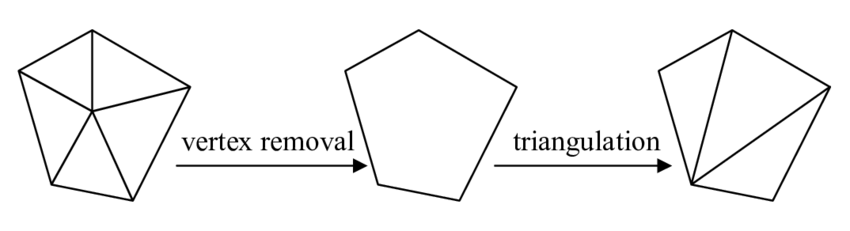
\includegraphics[scale=.48]{images/vertex-dec.png}  
    \end{center}

\end{frame}


\begin{frame}{Steps}
    \begin{center}
   
           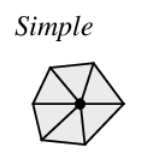
\includegraphics[scale=1.25]{images/simple.png}  
            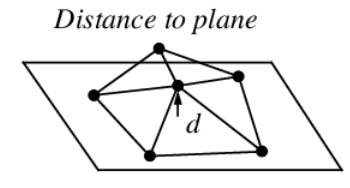
\includegraphics[scale=1.11]{images/distance.png}

    \end{center}

\end{frame}


\begin{frame}{Steps}
    \begin{center}
   
           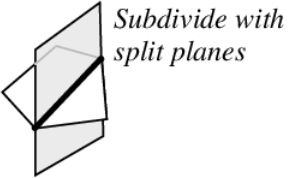
\includegraphics[scale=1.1]{images/split.png}  
            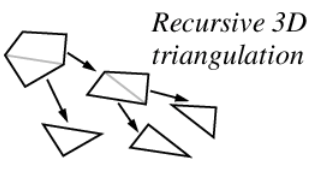
\includegraphics[scale=1.14]{images/recursion.png}

    \end{center}

\end{frame}